 \hypertarget{index_intro_sec}{}\subsection{Introduction}\label{index_intro_sec}
This project is about using an W\+S2811 or W\+S2812 lightstribe with an A\+V\+R controller. It is possible to handle up to 250 L\+E\+Ds at the same time, so I chose an Atmega328p with enough R\+A\+M amount. If you want to handle less L\+E\+Ds you can use most parts of this project with every A\+V\+R. The A\+V\+R is programmed to receive the light data over U\+A\+R\+T so you can control the L\+E\+Ds by using a serial interface. The interface uses a specified simple protocol which is described in \hyperlink{index_protocol_sec}{Protocol overview} section. Everything has been developed in a university course to control the lights of a Christmas tree. In the original implementation there were some further components included. This is a simplified version of the implementation so that everyone can use it. As an example for controlling the L\+E\+Ds using a smart phone the \hyperlink{index_esp_sec}{Example usage with an E\+S\+P8266} section shows how this could be done by using a webserver on the E\+S\+P8266. You can use everything else that provide a serial interface (maybe connect with a bluetooth serial module). The structure of this documentation is split in a hardware part for the A\+V\+R that describes the basic hardware that should be used. The next part is about how the software is working on the A\+V\+R that handles the L\+E\+Ds and different effects. You may include some more stuff in your own. After that you can see a small protocol overview, where you find which command can be sent to the A\+V\+R to control the L\+E\+Ds. Be aware that at the initialization state all L\+E\+Ds are off. At the last point you can find an example how to use the implementation with an E\+S\+P8266 with a webserver. You will find the source code for the E\+S\+P8266 and the basic hardware setup.\hypertarget{index_usage_sec}{}\subsection{Basic usage}\label{index_usage_sec}
For using this implementation follow this steps\+: 
\begin{DoxyItemize}
\item set up the hardware as descriped in section \hyperlink{index_hardware_sec}{Hardware} 
\item set the \hyperlink{globals_8h_a43bafb28b29491ec7f871319b5a3b2f8}{F\+\_\+\+C\+P\+U} clock to the value for your hardware 
\item set the \hyperlink{ws2811lichterkette_8c_a62634036639f88eece6fbf226b45f84b}{B\+A\+U\+D} to the value you like, 76800 or 38400 are suggested 
\item compile your implementation (only O1 optimization is supported) 
\item program your A\+V\+R with your binaries 
\item set the clock divider fuse and the clock source fuse referring to your implementation 
\item send protocol data (see section \hyperlink{index_protocol_sec}{Protocol overview}) to the R\+X pin of the A\+V\+R over a serial device, e.\+g. an F\+T\+D\+I, E\+S\+P8266 or Arduino (U\+A\+R\+T is 8\+N1 on your chosen \hyperlink{ws2811lichterkette_8c_a62634036639f88eece6fbf226b45f84b}{B\+A\+U\+D})(example data 254 6 0 1 20 22 = 0x\+F\+E 0x06 0x00 0x01 0x14 0x16) 
\end{DoxyItemize}\hypertarget{index_hardware_sec}{}\subsection{Hardware}\label{index_hardware_sec}
The basic hardware you need is a A\+V\+R controller an some W\+S2811 or W\+S2812 L\+E\+Ds you want to control. The A\+V\+R controller should have an hardware U\+A\+R\+T, otherwise you need to write some code for a software serial. In the project we chose an Atmega328p that has enough R\+A\+M to control 250 L\+E\+Ds. The internal software structure buffers the color data for the L\+E\+Ds to achieve an accurate timing, see section \hyperlink{index_software_sec}{Software implementation}. The A\+V\+R can be used with the internal clock at 8 M\+Hz, remember to clear the clock divider fuse. Otherwise an external 8 M\+Hz or 16 M\+Hz clock source can be used, the definition \hyperlink{globals_8h_a43bafb28b29491ec7f871319b5a3b2f8}{F\+\_\+\+C\+P\+U} must be set to the frequency you chose (remember to set the fuses for an external clock source). As an example \hyperlink{index_one}{figure 1} shows using an external 16 M\+Hz crystal. \label{index_one}%
\hypertarget{index_one}{}%
  
\begin{DoxyImage}
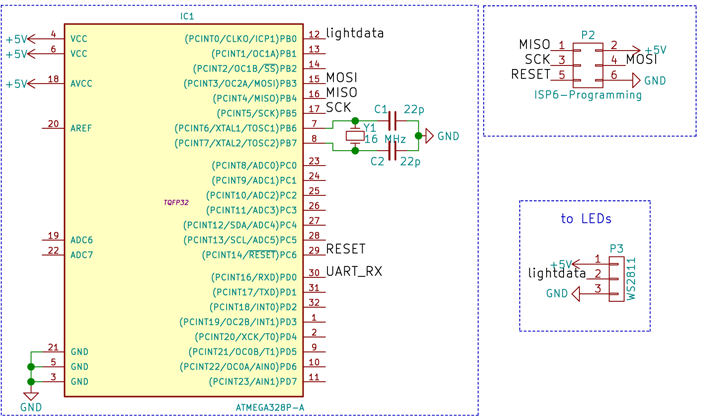
\includegraphics[width=\textwidth,height=\textheight/2,keepaspectratio=true]{Ws2811_Atmega328_schematic.png}
\caption{schematic of the A\+V\+R to controll W\+S2812/\+W\+S2811}
\end{DoxyImage}
  As you can see in the picture the A\+V\+R is programmed by using the I\+S\+P interface. The W\+S2812/\+W\+S2811 get the same voltage as the A\+V\+R, the light data is available at Pin\+B0, you may change this if you like. Referring to the L\+E\+Ds be aware of the current amount they may draw if every L\+E\+D has its full brightness. One W\+S2812 can draw up to 60 m\+A, so one meter with 30 L\+E\+Ds already need 1,8 A. If you want to control more L\+E\+Ds you may have a problem with the voltage drop along the stribe. For example if you control 180 L\+E\+Ds at six meters you not only need 10,8 A, furthermore you will probably have a voltage drop up to 2 V. To reduce the voltage drop you must increase the wire size with parallel wires to you stribe. You can see the voltage drop if you set all L\+E\+Ds to white. If you have only a small voltage drop every L\+E\+D will have the same color. If the voltage drop is too much you can see that the last L\+E\+Ds will have less blue color, so they will light in a warm white color even up to red. If you want to try out the L\+E\+Ds with the A\+V\+R you can build up everything on a breadboard. Pinheaders can be soldered easy at the light stribes as you can see in \hyperlink{index_two}{figure 2}. \label{index_two}%
\hypertarget{index_two}{}%
  
\begin{DoxyImage}
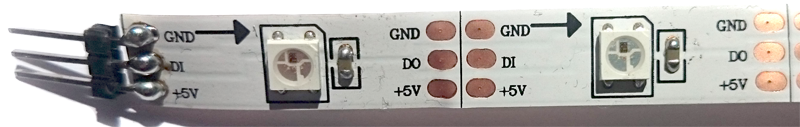
\includegraphics[width=\textwidth,height=\textheight/2,keepaspectratio=true]{WS2812.png}
\caption{W\+S2812 stribe with pin header}
\end{DoxyImage}
  The connect G\+N\+D to the common ground with the A\+V\+R, 5 V should be connected to a power supply that can handle the current you need. D\+I is the data in line, this should be connected to Pin\+B0 at the A\+V\+R. The stribe is like a big shifting register, all the data you sent is shifted bit by bit through the stribe. So D\+O is the data out pin, you see some data at this pin if all L\+E\+Ds before had already received their color data. The one wire protocol of the L\+E\+Ds is described in the next section \hyperlink{index_software_sec}{Software implementation}.

Datasheets\+:~\newline
 \href{WS2812.pdf}{\tt {\bfseries Datasheet W\+S2812}} ~\newline
 \href{WS2811.pdf}{\tt {\bfseries Datasheet W\+S2811}} ~\newline
 \href{Atmega328.pdf}{\tt {\bfseries Datasheet Atmega328}} ~\newline
\hypertarget{index_software_sec}{}\subsection{Software implementation}\label{index_software_sec}
If your hardware is ready you must flash your A\+V\+R device with the provided software. Therefore the I\+S\+P-\/6 connector should be used. To get the right timing remember to set the \hyperlink{globals_8h_a43bafb28b29491ec7f871319b5a3b2f8}{F\+\_\+\+C\+P\+U} definition to the frequency you are working at. Furthermore set the fuses of the A\+V\+R referring to your implementation. This means you have to clear the clock divider fuse and may have to change the clock source. I suggest to use the Atmel\+Studio to program your A\+V\+R and its fuses. ~\newline
 The W\+S2812/\+W\+S2811 are controlled by one data line that works with a one wire protocol. Because of the missing clock line the timing is really important, this can either be achieved by doing some trick with the hardware interfaces (e.\+g. using the spi interface) or by bit banging. In this implementation bit banging is used. To get a good timing all color data must be transmitted in one block that is not interrupted by some other code. The timing specifications of the W\+S2812/\+W\+S2811 L\+E\+Ds can be found in table \hyperlink{index_timingtable}{1} which refers to the datasheet ( \href{WS2812.pdf}{\tt {\bfseries W\+S2812}}).~\newline


\label{index_timingtable}%
\hypertarget{index_timingtable}{}%
 \begin{table}[h]\begin{TabularC}{3}
\hline
\rowcolor{lightgray}{\bf Information }&{\bf Timing }&{\bf Tolerance +/-\/ }\\\cline{1-3}
Transfer 1 Bit &High\+Time+\+Low\+Time=1,25 µs &600 ns \\\cline{1-3}
send 0, high time &0,35 µs &150 ns \\\cline{1-3}
send 0, low time &0,8 µs &150 ns \\\cline{1-3}
send 1, high time &0,7 µs &150 ns \\\cline{1-3}
send 1, low time &0,6 µs &150 ns \\\cline{1-3}
data transmission complete, low time &$>$50 µs &-\/ \\\cline{1-3}
\end{TabularC}
\centering
\caption{Timing table for W\+S2812/\+W\+S2811 one wire protocol}
\end{table}


The timing is done by setting the output and wait the required time by doing nothing (call assembly N\+O\+Ps). So it is important to compile the provided software at O1, other optimization levels may influence the timing. To send one bit (either high or low) two different macros are defined in \hyperlink{_lightstribe_8h}{Lightstribe.\+h} (S\+E\+T\+H\+I\+G\+H and S\+E\+T\+L\+O\+W), one L\+E\+D needs 24 color bits. The macros depend on the value of \hyperlink{globals_8h_a43bafb28b29491ec7f871319b5a3b2f8}{F\+\_\+\+C\+P\+U} you entered in \hyperlink{globals_8h}{globals.\+h}. Furthermore the header file Lightstrib.\+h declares a color struct to handle 24 bit colors (\hyperlink{structcolor24bit}{color24bit}) and three basic functions to control the L\+E\+Ds. The corresponding c file \hyperlink{_lightstribe_8c}{Lightstribe.\+c} implements these functions. The most important function is the \hyperlink{_lightstribe_8h_aac724dad670e4a26723daf71ce6a8d8a}{transmit2leds} function. This function and only this function transmits data to the stribe. All other functions either call this function or manipulate the color array. To achieve the right timing all effects and operations are done on a color array that stores the color information for the L\+E\+Ds. The information is sent to the L\+E\+Ds by calling transmit2leds with the lightdata pointer that points to an dynamically allocated array that stores the color information depending on the number of L\+E\+Ds you want to control. Therefore your color array must at least be able to contain 24 bits x your number of L\+E\+Ds. It can be bigger, what will allow you to create even more effects (e.\+g. if you rotate a rainbow array). So the effects that are implemented in \hyperlink{_led_effects_8c}{Led\+Effects.\+c} change the color array and afterwards the \hyperlink{_lightstribe_8h_aac724dad670e4a26723daf71ce6a8d8a}{transmit2leds} is called. The c file \hyperlink{_led_effects_8c}{Led\+Effects.\+c} not only contains effects but also different necessary functions for the effects and the serial color handling. The \hyperlink{_led_effects_8h_a55291315ab0f2ca8d508f0e9da1920a7}{colorconv8to24} function converts the received 8 bit colors from the serial port to 24 bit colors for the lightstribes. So you only sent 8 bit colors over the serial port to the A\+V\+R to reduce data size. Further information can be found in the \hyperlink{index_protocol_sec}{Protocol overview} section. The colors are decompressed with a simple \hyperlink{_led_effects_8h_ad67a4e660b5122ed454e101432bbdba0}{map} function you may know from Arduino. The main.\+c file initializes the hardware and handles the L\+E\+Ds. A serial interrupt stores the data temporary. If the data transmission is complete the main function will extract the information and set the new configuration for the lightstribe.~\newline
 The last points to be mentioned in this section are some things you need to be careful. The first thing is that the 8 bit colors are in an R\+G\+B 3-\/3-\/2 format. The 24 bit color format depend on the L\+E\+Ds. W\+S2812 L\+E\+Ds use a G\+R\+B color scheme while W\+S2811 use a R\+G\+B color scheme. This is important, to achieve the right color the protocol includes a bit that decides the color scheme. The right color is resolved by the decompressing function \hyperlink{_led_effects_8h_a55291315ab0f2ca8d508f0e9da1920a7}{colorconv8to24}. Another thing is that the colors are not linearized, what means that you cannot say that a color you got from a color table will be look like this. As an example you picked an orange from a 3-\/3-\/2 rgb color table. This orange will not be the same orange on the L\+E\+D stribe. This depends on many parameters so linearizing is too much effort and almost impossible (to achieve linearization you would have to measure each color, compare it and evaluate correction parameters).\hypertarget{index_protocol_sec}{}\subsection{Protocol overview}\label{index_protocol_sec}
This section gives an overview of the implemented serial protocol. The goal of the protocol was to be as simple as possible, to be easily implemented on the A\+V\+R and to use as less resources as possible. \hyperlink{index_three}{Figure 3} shows the base structure of the protocol. \label{index_three}%
\hypertarget{index_three}{}%
  
\begin{DoxyImage}
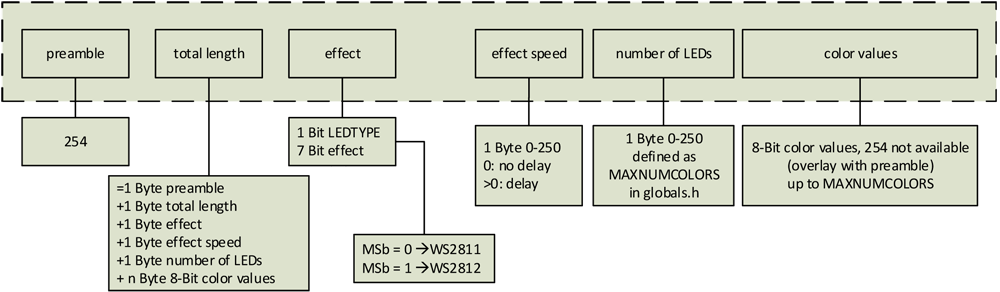
\includegraphics[width=\textwidth,height=\textheight/2,keepaspectratio=true]{Protoll_V1_2_engl.png}
\caption{serial protocol structure}
\end{DoxyImage}
 As you can see a data transmission always starts with the preamble 254(0x\+F\+E). For a fast and easy implementation this preamble value must only be used as preamble and must never be another field value (e.\+g. you must not send the color value 254). The next byte that is sent contains the total length of the packet including the preamble and the length byte. If you sent a wrong length you may get an unexpected behavior until a new correct data packet is sent. The third field contains the effect. The different effects are listed in table X\+X\+X. In Bit 7 (M\+Sb) you can choose the L\+E\+D type you want to control, set the bit to 0 for W\+S2811 and to 1 for W\+S2812 L\+E\+Ds. The next byte is a value to control the effect speed. You can set a delay between 0 (no delay) and 250 (longest delay possible). The value unit and is not a repeatable setting for different effects. This means that the delay is no correct wait function (e.\+g. wait for n milliseconds). Furthermore the effects work on the color array what may be faster for some effects and slower for others. The best thing is to try the effects with different values. The next field contains the number of the L\+E\+Ds that should be controlled. Be aware that the maximum supported number of L\+E\+Ds is 250, but this depends on your hardware. The chosen Atmega328p can handle this amount, if you choose an A\+V\+R with less R\+A\+M this will not work. What you can do is to allocate more L\+E\+Ds than you actually have. This gives you the possibility to create further effects. What happens is that only a part of the array is sent to the L\+E\+Ds but the other color values are stored internally in the A\+V\+R (in fact all color data is transmitted to the L\+E\+Ds but the superfluous information is overwritten by new data). The last data field are the color values. One color is 8 bit R\+G\+B 3-\/3-\/2 and you should sent the right amount of colors for your chosen effect. If you sent to less information the data block will not be evaluated because the total length does not match. For sending some data do not forget to configure your U\+A\+R\+T (8\+N1 \hyperlink{ws2811lichterkette_8c_a62634036639f88eece6fbf226b45f84b}{B\+A\+U\+D}) on both sides.

\label{index_effecttable}%
\hypertarget{index_effecttable}{}%
 \begin{table}[h]\begin{TabularC}{4}
\hline
\rowcolor{lightgray}{\bf Effect~\newline
number }&{\bf Number of colors ~\newline
 (1 byte R\+G\+B 3-\/3-\/2) }&{\bf Description }&{\bf Example ~\newline
 (decimal) }\\\cline{1-4}
0 = S\+E\+T\+F\+U\+L\+L\+C\+O\+L\+O\+R &1 &All L\+E\+Ds glow at the same color without changes. &254 6 1 20 22 \\\cline{1-4}
1 = F\+I\+L\+L\+U\+P &2 (foreground, background) &One L\+E\+D steps through the stribe in the foreground color and colors all L\+E\+Ds after it in the background color.~\newline
 At the end of the stribe the L\+E\+D stays at the foreground color and another L\+E\+D starts to step through the stribe.~\newline
 This continues until the whole stribe is filled in the foreground color. ~\newline
 Then the stribe is cleared to the background color and the effects begins again. &254 7 1 22 20 22 201 \\\cline{1-4}
2 = B\+L\+I\+N\+K &1 &The stribe blinks in the chosen color and to off (=black) repeatedly. &254 6 2 55 20 56 \\\cline{1-4}
3 = R\+U\+N\+L\+E\+D &2 (foreground, background) &All L\+E\+Ds but one are colored in the background color.~\newline
 The one in the foreground color walks through the stribe with overflowing to the beginning. &254 7 3 55 20 56 151 \\\cline{1-4}
5 = A\+L\+T\+E\+R\+N\+A\+T\+E &2 (foreground, background) &The L\+E\+Ds are alternating in the foreground and the background color.~\newline
 First the even L\+E\+Ds are colored in foreground and the uneven in the background color, after that vice versa. &254 7 5 55 20 56 151 \\\cline{1-4}
7 = R\+E\+C\+O\+L\+O\+R &1 &The stribe is filled in a new color step by step until the whole stribe stays in the new color. &254 6 7 55 20 38 \\\cline{1-4}
8 = F\+A\+D\+E &1 &The destination color is set and the base colors red, green and blue are decreased step by step until the stribe is off.~\newline
 After that the color values are increased until the destination color is reached.~\newline
 This generates a color fading effect. The color fading is not linearized. &254 6 8 55 20 201 \\\cline{1-4}
9 = I\+N\+I\+T\+R\+A\+I\+N\+B\+O\+W &no color &Set the stribe in a static rainbow color. &254 5 9 0 20 \\\cline{1-4}
10 = R\+O\+T\+A\+T\+E\+\_\+\+R &no color &Rotate all L\+E\+Ds one step to the right side (depends on lightdata array). &254 5 10 232 20 \\\cline{1-4}
11 = R\+O\+T\+A\+T\+E\+\_\+\+L &no color &Rotate all L\+E\+Ds one step to the left side (depends on lightdata array). &254 5 11 23 20 \\\cline{1-4}
12 = C\+U\+S\+T\+O\+M &N colors &All L\+E\+Ds are set to the static color referring to the sent color values.~\newline
 If there are more L\+E\+Ds than color values the colors are repeated. &254 8 12 1 20 22 201 60 \\\cline{1-4}
\end{TabularC}
\centering
\caption{Table containing all effects available over the serial protocol}
\end{table}
The missing numbers in table \hyperlink{index_effecttable}{2} are internally used by the A\+V\+R and must not be sent over the serial port.\hypertarget{index_owneffects_sec}{}\subsection{Implement further effects}\label{index_owneffects_sec}
This section tells you how to implement further effects. You may use already existing functions to generate new effects or add something completely new. All effects should be written in the \hyperlink{_led_effects_8c}{Led\+Effects.\+c} file and declared in its header file \hyperlink{_led_effects_8h}{Led\+Effects.\+h}. You must know that everything works on a lightdata array that contains the colors stored in an array. The array is sent directly to the stribe if the \hyperlink{_lightstribe_8h_aac724dad670e4a26723daf71ce6a8d8a}{transmit2leds} function is called. So you first need to manipulate the array and than send it to the stribe. The array is ordered in G\+R\+B color because the implementation has been done for W\+S2812 L\+E\+Ds (W\+S2811 L\+E\+Ds can be used the colors are converted in the \hyperlink{_led_effects_8h_a55291315ab0f2ca8d508f0e9da1920a7}{colorconv8to24} function referring to the M\+Sb of the effect you sent, for more information see section \hyperlink{index_protocol_sec}{Protocol overview}). So lightdata\mbox{[}0\mbox{]} contains one byte green data, lightdata\mbox{[}1\mbox{]} one byte red data, lightdata\mbox{[}2\mbox{]} blue data and so on. In general you can say lightdata\mbox{[}N\%3==0\mbox{]} contains green, lightdata\mbox{[}N\%3==1\mbox{]}, lightdata\mbox{[}N\%3==2\mbox{]} data. So the color array has a size of \hyperlink{globals_8h_a6e2b9e79df9491377ae405ef85aa0ca5}{M\+A\+X\+N\+U\+M\+C\+O\+L\+O\+R\+S} $\ast$ 3. So your function must at least have a pointer to the lightdata array as a call value. For creating your effect some nice functions are already implemented you may use. You can find a list of them in table \hyperlink{index_functiontable}{3}.

\label{index_functiontable}%
\hypertarget{index_functiontable}{}%
 \begin{table}[h]\begin{TabularC}{3}
\hline
\rowcolor{lightgray}{\bf Function Name }&{\bf call values }&{\bf operation }\\\cline{1-3}
\hyperlink{_led_effects_8h_ad67a4e660b5122ed454e101432bbdba0}{map} &x,in\+\_\+min,in\+\_\+max,out\+\_\+min,out\+\_\+max &calculate an x value to a new number range \\\cline{1-3}
\hyperlink{_led_effects_8h_a6950e7657ba74d0d490ba36427533c4b}{effectdelay} &delay &wait some time dependend on delay \\\cline{1-3}
\hyperlink{_led_effects_8h_a1c5e6b0f45c1787c25f8eafa8b9c6247}{resetstribe} &$\ast$lightdata &clear the stribe (all L\+E\+Ds off) \\\cline{1-3}
\hyperlink{_led_effects_8h_afd64325b08e785d37b4dfaf358e517f0}{rotate} &$\ast$lightdata, direction &rotate stribe by one position (means 3 bytes) in direction (right/left) \\\cline{1-3}
\hyperlink{_led_effects_8h_a1fa5e03cb24195a46dcdc5948f596181}{rotate\+N} &$\ast$lightdata, direction,width &rotate L\+E\+Ds by \char`\"{}width\char`\"{} positions (means width $\ast$ 3 bytes) in direction (right/left) \\\cline{1-3}
\hyperlink{_lightstribe_8h_abba9462833e30ef725eaf18c3d01eb71}{setled} &color, $\ast$lightdata, lednr &set one L\+E\+D a position lednr in the chosen color, others off (black) \\\cline{1-3}
\hyperlink{_lightstribe_8h_a63fa595d401f0e85c1bba55ba2b1d66e}{changeled} &color, $\ast$lightdata, lednr &change the color of one L\+E\+D at position lednr, others are unchanged \\\cline{1-3}
\end{TabularC}
\centering
\caption{Provided help functions for your own effect}
\end{table}


Your written effect should get an own definition in \hyperlink{_led_effects_8h}{Led\+Effects.\+h} . The last thing is to add your definition in the main switch case structure. Referring to the implemented protocol your effect is available with the number you defined in \hyperlink{_led_effects_8h}{Led\+Effects.\+h}. You must sent the neccessary information for your effect, for example the color values you need and so on. To get the color value you sent you need to call \hyperlink{_led_effects_8h_a55291315ab0f2ca8d508f0e9da1920a7}{colorconv8to24} to convert the 8 bit R\+G\+B color into a 24 bit color. All colors you sent are available in the \hyperlink{globals_8h_a159854edb9d0c7283013495d85bdf997}{Comp\+Color\+Array}. The first color you sent is stored in index zero. Your implemented function must not care about the color order if you use the \hyperlink{_led_effects_8h_a55291315ab0f2ca8d508f0e9da1920a7}{colorconv8to24} function. This does the conversion depending on the M\+Sb of the effect you sent over the serial port. The delay is handled by the global var \hyperlink{globals_8h_ac2445d316b2972d381edeac44bb6a226}{effectime} and the number of L\+E\+Ds to control is stored in \hyperlink{globals_8h_ad5db4045aed262ed4aae2af9d81fab98}{Num\+Of\+Leds}. The effect is stored in the \hyperlink{globals_8h_a053b8e1f039c19251b90d60317db8aed}{effect} variable. You should not do any changes on the serial part and the protocol reading, otherwise you will change to complete behavior of this implementation.\hypertarget{index_limitations_sec}{}\subsection{Requirements and Limitations}\label{index_limitations_sec}
The implementation to control has the following requirements and limitations\+: 
\begin{DoxyItemize}
\item colors are 8 bit compressed so you cannot get every color value of the L\+E\+Ds 
\item the protocol implementation with the preamble 254 prohibits this value for other protocol fields (e.\+g. color) 
\item approximate amount of R\+A\+M (in bytes) you need\+: \hyperlink{globals_8h_a6e2b9e79df9491377ae405ef85aa0ca5}{M\+A\+X\+N\+U\+M\+C\+O\+L\+O\+R\+S}(=number of L\+E\+Ds to control)$\ast$3 + \hyperlink{globals_8h_a0d57378e32bf8278011460740bc29f7f}{U\+A\+R\+T\+\_\+\+B\+U\+F\+F\+E\+R\+\_\+\+S\+I\+Z\+E} $\ast$2 + \hyperlink{globals_8h_a6e2b9e79df9491377ae405ef85aa0ca5}{M\+A\+X\+N\+U\+M\+C\+O\+L\+O\+R\+S} + 160 
\item only O1 optimization is supported 
\item 8 M\+Hz and 16 M\+Hz clock support 
\item fuses must be programmed manually (clock source and clock divider) 
\item W\+S2801 stribes not supported (different hardware interface with two wires) 
\item A\+V\+R should run on 5 V 
\end{DoxyItemize}\hypertarget{index_esp_sec}{}\subsection{Example usage with an E\+S\+P8266}\label{index_esp_sec}
This section gives a short introduction about using the provided programm with an E\+S\+P8266. In this example the E\+S\+P8266 works as a wifi hotspot you can connect with and browse a website which allows different settings for the light stribe. The website is quite simple and only a few effects and colors are supported. If you enter the button \char`\"{}\+D\+O I\+T\char`\"{} your configuration is transmitted over the serial interface to the A\+V\+R. This is done through a software serial implementation, you find all necessary files below. You should step through all instructions to get the example work.\hypertarget{index_setup_esp}{}\subsubsection{E\+S\+P8266 setup}\label{index_setup_esp}
First you need to setup the E\+S\+P8266. Because of different versions of E\+S\+P8266 modules you may miss something, this is just a quick guide. For more information you can browse the web. First you must connect your E\+S\+P8266 to a host computer over a serial interface for example using an F\+T\+D\+I. Remember to cross R\+X and T\+X of the serial port. Furthermore be aware of the E\+S\+P8266 voltage, it is 3,3 V. The current a serial chip may provide (some F\+T\+D\+Is provide some current) may not be enough for the E\+S\+P8266 and what can cause different problems. ~\newline
 So first you need to flash your E\+S\+P8266 with the nodemcu firmware that provides a software serial. The binaries that have been used in this example can be found here\+: ~\newline
 \href{0x00000.bin}{\tt {\bfseries Binaries part 1}} ~\newline
 \href{0x10000.bin}{\tt {\bfseries Binaries part 2}} ~\newline
 For uploading this binaries to the E\+S\+P8266 you should use the \href{https://github.com/nodemcu/nodemcu-flasher}{\tt node\+M\+C\+U\+Flasher} that can be found on github. You need to set the serial port to which your E\+S\+P8266 is connected with and configure the source files for flashing the firmware. You need to set the C\+O\+M port to which you E\+S\+P8266 is connected to (see \hyperlink{index_four}{figure 4}). Furthermore you must consider the following hardware configuration\+: 
\begin{DoxyItemize}
\item 3,3 V logic level 
\item bootmode low (I\+O15) 
\item chip enable high (C\+H\+\_\+\+P\+D) 
\item reset high (drive low to reset the module) 
\item I\+O0 low for firmware flashing (high for programming and normal operation) 
\end{DoxyItemize}The firmware programmer waits for the M\+A\+C of the E\+S\+P8266 module which will be successfully read if everything is done fine. As you can see in \hyperlink{index_four}{figure 4} the firmware programmer is still waiting for an E\+S\+P8266. \label{index_four}%
\hypertarget{index_four}{}%

\begin{DoxyImage}
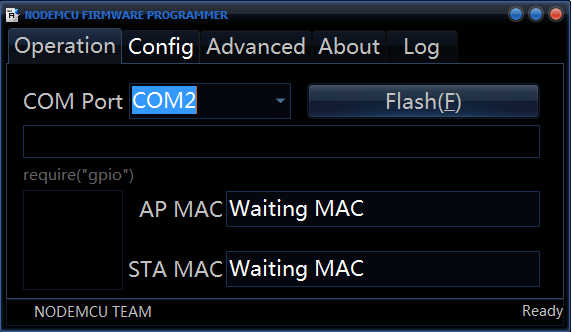
\includegraphics[width=\textwidth,height=\textheight/2,keepaspectratio=true]{NodeMCUFlasher_flash.PNG}
\caption{serial protocol structure}
\end{DoxyImage}
If the E\+S\+P8266 is connected right you now set the configuration to the provided binaries as you can see in \hyperlink{index_five}{figure 5}. You must browse to the binary files and set the destination address. Now you can hit the \char`\"{}\+Flash\char`\"{}-\/\+Button (see \hyperlink{index_four}{figure 4}). \label{index_five}%
\hypertarget{index_five}{}%

\begin{DoxyImage}
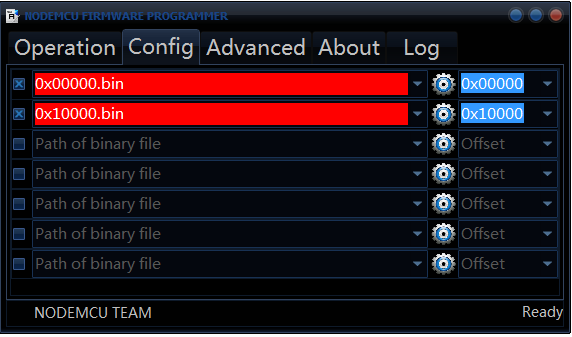
\includegraphics[width=\textwidth,height=\textheight/2,keepaspectratio=true]{NodeMCUFlasher_config.PNG}
\caption{serial protocol structure}
\end{DoxyImage}
After flashing the firmware you need to reboot the E\+S\+P8266 module. Before you do this you should change the I\+O0 to high level (3\+V3) because after the reboot we want to program the module with our own program. The reset can be done by setting reset low. The program we will upload to the module is written in Lua. Lua is a scripting language that is interpreted by the firmware running on the module. So the performance is not the best, but the programming is quite simple. The little program that you can find below set up the module as an access point, runs a simple webserver that interacts with a software serial to control the A\+V\+R. One thing you must know about the Lua programming is that the variable types are assigned implicit so you cannot control whether a number is stored as 16 bit or 32 bit signed or unsigned variable. Another thing you should know is that the program you write needs the full memory space of its file. That means shorter variable names save memory and furthermore documentation should be as short as possible or left.~\newline
 For writing your program you can use any text editor, notepad++ is a good choice. If you are finished you must upload the file to the module. Therefore you use the same setup as for firmware updating but you must set I\+O0 to high level. For uploading your program you can use the E\+S\+P8266 Lua Loader. It is easy to handle and you can try out several things first, before you upload your code. You can find the main window of the E\+S\+P8266 Lua Loader in \hyperlink{index_six}{figure 6}. \label{index_six}%
\hypertarget{index_six}{}%

\begin{DoxyImage}
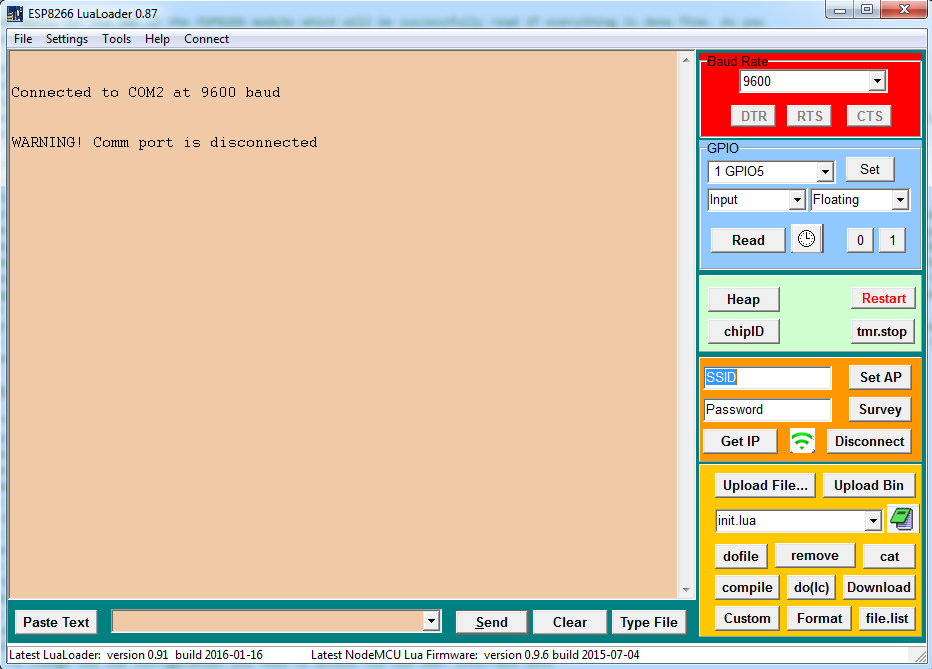
\includegraphics[width=\textwidth,height=\textheight/2,keepaspectratio=true]{LuaLoader.png}
\caption{E\+S\+P8266 Lua Loader}
\end{DoxyImage}
On the right side you can set the baud rate for uploading you program to the module. In the G\+P\+I\+O section you can easily set and reset them to try your wiring. By using the restart button you will restart the module. This may be necessary if your heap (R\+A\+M) is to low. This is caused by inefficient programming or by a program that is to big for the module. Global variables need a lot of heap. For uploading your program hit the \char`\"{}\+Upload File...\char`\"{} button. In a file browser you choose your program that should be transferred to the module. After completion you hit the \char`\"{}dofile\char`\"{} button to run the program. This short description should be enough.~\newline
 So now we upload the Lua program that starts the webserver and sends data over a software serial to the A\+V\+R. You can find this program here\+:~\newline
 \href{complex_server.lua}{\tt {\bfseries lua program for controlling the A\+V\+R}} ~\newline
 The program does the following\+: 
\begin{DoxyItemize}
\item set up the E\+S\+P8266 module as an access point (S\+S\+I\+D=Lichterkette, password=12345678, you may change this) 
\item start a webserver that listens on port 80 
\item load the index.\+html website and handle requests 
\item sent U\+A\+R\+T commands matching for the A\+V\+R implementation to generate different effects depending on the request 
\item software serial is set to G\+P\+I\+O5 (G\+P\+I\+O5 is available at software number 1) 
\end{DoxyItemize}Some further things you should know\+: 
\begin{DoxyItemize}
\item the maximum of parallel accessing devices is four 
\item parallel devices can never access another device 
\item the software uart only supports T\+X (8\+N1 up to 38400 baud) 
\item if you change the website you must change the hard coded content length of the website 
\item the address of the E\+S\+P8266 is always 192.\+168.\+4.\+1 
\end{DoxyItemize}\hypertarget{index_avr_con_esp}{}\subsubsection{Connect E\+S\+P8266 with A\+V\+R}\label{index_avr_con_esp}
After uploading the main program file you need to upload the \href{_index.html}{\tt {\bfseries \+\_\+index.\+html}} file. Before uploading remove the underscore so that the files name is index.\+html (the underscore has been inserted because of conflicts with this html documentation). For uploading other file types (than lua programs) to your E\+S\+P8266 module you need to use the \char`\"{}\+Upload Bin\char`\"{} button of the Lua Loader. The file will be uploaded to the file system on the E\+S\+P8266. ~\newline
 Now your E\+S\+P8266 module is ready to try the first communication with the A\+V\+R. So now you need a hardware setup where the E\+S\+P8266 and A\+V\+R are connected. Be aware of the different voltage levels (A\+V\+R uses 5\+V, E\+S\+P8266 3\+V3). You should connect everything like \hyperlink{index_seven}{figure 7} shows.

\label{index_seven}%
\hypertarget{index_seven}{}%

\begin{DoxyImage}
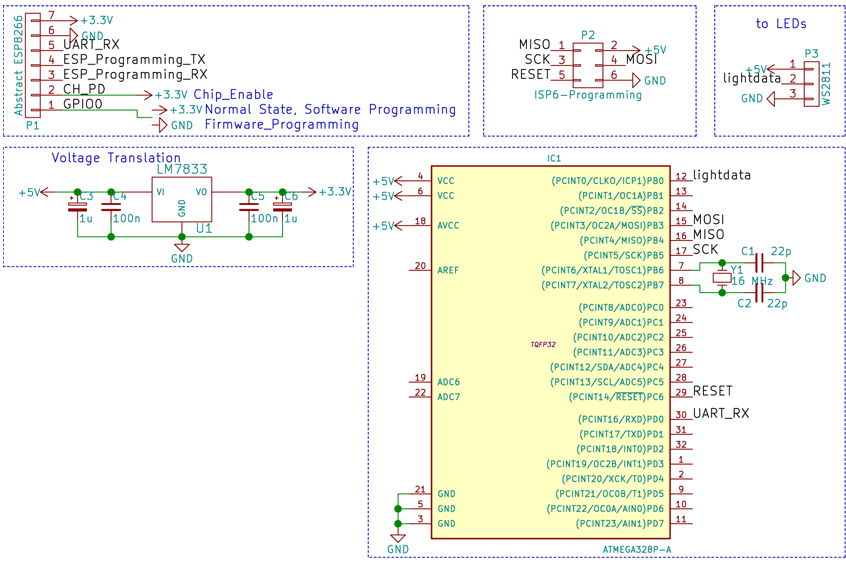
\includegraphics[width=\textwidth,height=\textheight/2,keepaspectratio=true]{Ws2811_Atmega328.png}
\caption{schematic using E\+S\+P8266 with A\+V\+R W\+S2811 software}
\end{DoxyImage}
 Your E\+S\+P8266 should still be connected with the host computer. If your hardware setup is ready you now must hit the \char`\"{}dofile\char`\"{} button in the Lua Loader (complexe\+\_\+server.\+lua must be the selected file that should be executed). After a short time you can use any device to search for the access point that is set up by the E\+S\+P8266 module. It will have your S\+S\+I\+D (default \char`\"{}\+Lichterkette\char`\"{}) and your chosen password (default \char`\"{}12345678\char`\"{}). After you connected to your E\+S\+P8266 module you should open a web browser and browse the I\+P address 192.\+168.\+4.\+1. The browser should load the website. Now choose your configuration for the L\+E\+Ds and hit the \char`\"{}\+D\+O I\+T\char`\"{} Button on the website. The website should be reloaded and the lightstribes get the configuration you have chosen. If everything is working fine the last thing to do is to make the E\+S\+P8266 as a stand alone device without the need of an external host. For this you must remove the complex\+\_\+webserver.\+lua file from the module. Now you rename the file on your host computer to init.\+lua. Afterwards you upload this file to the E\+S\+P8266. This file is always loaded at first when the E\+S\+P8266 is powered on. So now you have a stand alone webserver that communicates with your A\+V\+R for controlling W\+S2811/\+W\+S2812 L\+E\+Ds.~\newline
\hypertarget{index_short_setup}{}\subsubsection{Short setup}\label{index_short_setup}

\begin{DoxyItemize}
\item flash the provided image (\href{0x00000.bin}{\tt {\bfseries Binaries part 1}},\href{0x10000.bin}{\tt {\bfseries Binaries part 2}} 
\item upload the \href{_index.html}{\tt {\bfseries \+\_\+index.\+html}} renamed to index.\+html 
\item upload the lua program \href{complex_server.lua}{\tt {\bfseries complex\+\_\+server.\+lua}} renamed to init.\+lua 
\item setup your hardware refering to \hyperlink{index_seven}{figure 7} 
\item connect to your E\+S\+P8266 with your S\+S\+I\+D and your password (default\+: Lichterkette, 12345678) 
\item browse 192.\+168.\+4.\+1 on your device 
\item set up your configuration and hit \char`\"{}\+D\+O I\+T\char`\"{} 
\end{DoxyItemize}~\newline
 author\+: Florian Wank, 2016 